\documentclass[titlepage,a4paper,12pt]{article}

% Match the Chinese manual's page geometry and code-box style.
\usepackage{fontspec}
\setmonofont{lmmono10-regular.otf}
\usepackage{geometry}
\geometry{a4paper,left=3.18cm,right=3.18cm,top=2.54cm,bottom=2.54cm}
\usepackage{graphicx}
\usepackage{float}
\usepackage{amsmath,amssymb}
\usepackage{indentfirst}
\usepackage[dvipsnames]{xcolor}
\usepackage{listings}
\usepackage{enumitem}
\usepackage{etoolbox}
\usepackage[hidelinks]{hyperref}
\setlength{\emergencystretch}{2em}

\lstset{
  basicstyle={\sffamily\footnotesize},
  numbersep=5pt,
  breaklines=true,
  captionpos={T},
  frame={lines},
  framerule=0.5pt,
  columns=flexible,
  tabsize=2,
  numbers=left,
  backgroundcolor={\color{yellow!3!white}}
}

% Keep each short example, including its closing bracket, on one page.
\BeforeBeginEnvironment{lstlisting}{\par\noindent\begin{minipage}{\linewidth}}
\AfterEndEnvironment{lstlisting}{\end{minipage}\par}
\newcommand\litem[1]{\item{#1?\\}}

\begin{document}
\title{\textsf{MagneticTB} manual}
\author{Zeying Zhang}
\maketitle
\tableofcontents

\begin{quote}
\small
This manual introduces the commonly used features of \textsf{MagneticTB} 2.0.
For a first calculation, install the package and follow the graphene example
in Section~\ref{gra}, running the code in order.
\end{quote}
\newpage

\section{Features}
\textsf{MagneticTB} is an open-source package based on the corepresentation theory
of magnetic groups. It constructs tight-binding models from crystal symmetry
and local orbitals. To define a model, provide the lattice vectors, Wyckoff
positions, magnetic moments, symmetry operations, and basis functions.
With these inputs, the package generates the symmetry-allowed Hamiltonian.
You can then assign parameter values and plot the bands. Its features include:
\begin{itemize}
\item Obtaining symmetry operations of magnetic space, layer, and rod groups.
\item Constructing models of magnetic and nonmagnetic materials, including
noncollinear magnetic structures.
\item Constructing spinless models and double-group models with spin-orbit coupling.
\item Starting from local orbitals at a reference site and using an induced
representation to construct basis functions at equivalent sites.
\item Plotting crystal structures, magnetic moments, first Brillouin zones, and
bands, including interactive band plots with adjustable parameters.
\item Reading and writing Wannier90 files, and working with band-fitting and
band-corepresentation tools.
\end{itemize}

\section{Installation, updates, and uninstallation}
\subsection{Installing and loading the package}
Once you have a local \lstinline|.paclet| file, run this command in Mathematica:
\begin{lstlisting}[numbers=none]
PacletInstall["/absolute/path/MagneticTB-2.0.10.paclet"]
\end{lstlisting}
Replace the path and filename with those of your file. On Windows, forward
slashes can also be used in paths, for example
\lstinline|"C:/Users/yourname/Downloads/MagneticTB-2.0.10.paclet"|.

Save your open notebooks, then \textbf{quit and reopen Mathematica completely},
rather than only restarting the kernel. After reopening Mathematica, load the
package:
\begin{lstlisting}[numbers=none]
Needs["MagneticTB`"]
\end{lstlisting}
This loads the functions. You still need to define a model with \lstinline|init|
before calling \lstinline|symham|.

\subsection{Opening the documentation}
Search for \textsf{MagneticTB} in Mathematica's Documentation Center, or run:
\begin{lstlisting}[numbers=none]
SystemOpen["paclet:MagneticTB/guide/MagneticTB"]
\end{lstlisting}
This opens the help home page shown in Figure~\ref{fig:help-home}.
Start with \emph{Getting started with MagneticTB} for installation, loading,
and a first model. Scroll down to browse the functions by topic.
\begin{figure}[H]
\centering
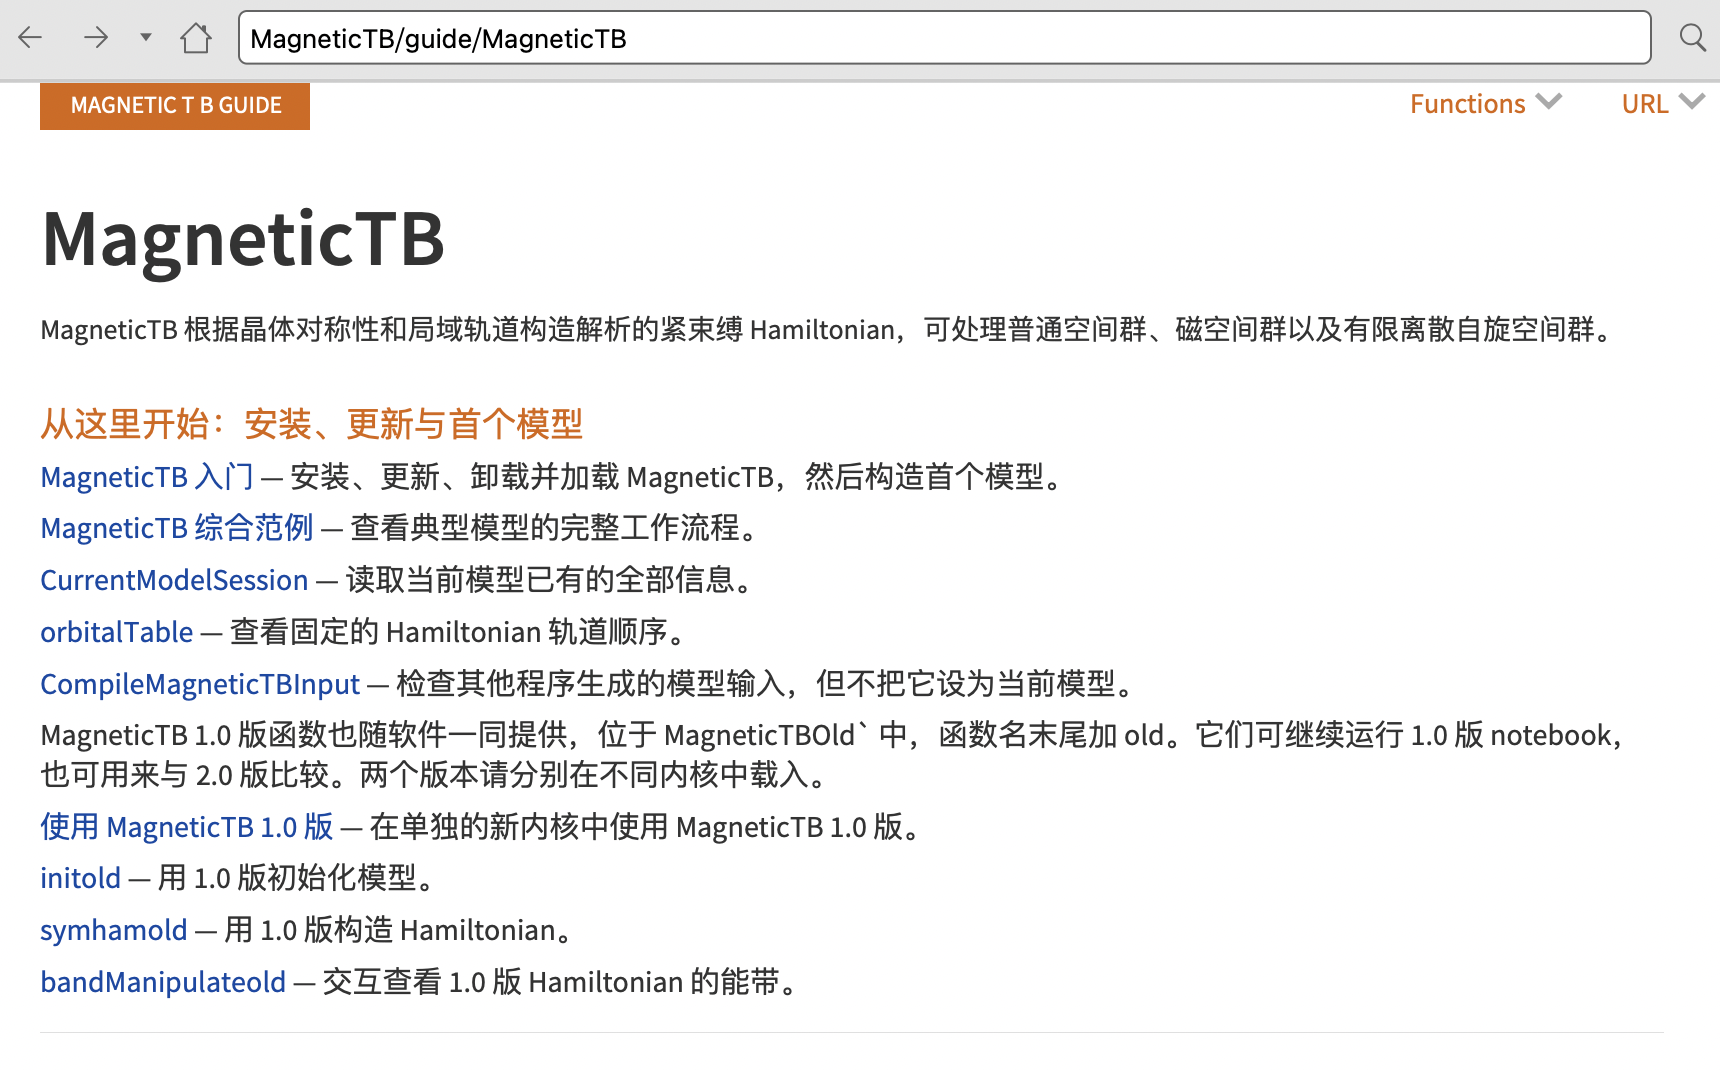
\includegraphics[width=\textwidth]{figures/manual-help-home.png}
\caption{The MagneticTB help home page in Mathematica, shown with the
Simplified Chinese interface. Click a blue link to open a tutorial or function page.
(The author purchased the Chinese-language version of Mathematica, so an
English-interface screenshot is not available.)}
\label{fig:help-home}
\end{figure}
To go directly to the initialization reference page, for example, run:
\begin{lstlisting}[numbers=none]
SystemOpen["paclet:MagneticTB/ref/init"]
\end{lstlisting}
The figures in this manual are static. Use Mathematica to operate the sliders
in \lstinline|bandManipulate|.

\subsection{Updating}
To update, install a local file with a higher version number:
\begin{lstlisting}[numbers=none]
PacletInstall["/absolute/path/MagneticTB-<new-version>.paclet"]
\end{lstlisting}
Then save your work, quit Mathematica completely, and reopen it.
Use \lstinline|PacletFind["MagneticTB"]| to see the installed versions.
Automatic online updates are not currently provided.

The message \lstinline|PacletInstall::samevers| means that this version is
already installed. If you need to reinstall the same version, uninstall it first:
\begin{lstlisting}[numbers=none]
PacletUninstall["MagneticTB"]
PacletInstall["/absolute/path/MagneticTB-2.0.10.paclet"]
\end{lstlisting}

\subsection{Uninstalling}
To remove the package, run:
\begin{lstlisting}[numbers=none]
PacletUninstall["MagneticTB"]
\end{lstlisting}
This uninstalls the package, but does not delete your own model notebooks.
Quit and reopen Mathematica afterwards so that you do not continue using
definitions already loaded in the kernel.

\section{Using MagneticTB}
\subsection{Obtaining symmetry operations}
Three functions form the main modeling workflow:
\lstinline|msgop| obtains the symmetry operations, \lstinline|init| sets up the
model, and \lstinline|symham| constructs the Hamiltonian.

For a nonmagnetic material, one normally uses a gray group, which includes
time-reversal symmetry. For example:
\begin{lstlisting}
Needs["MagneticTB`"];
sgop = msgop[gray[191]];
\end{lstlisting}
Here \lstinline|gray[191]| gives the identifier of the gray group associated
with space group 191, and \lstinline|msgop| converts that identifier into the
complete list of symmetry operations. It also prints the BNS number, group
symbol, and lattice vectors. To specify a magnetic group by its BNS number,
such as $191.239$, use:
\begin{lstlisting}[numbers=none]
msgop[bnsdict[{191, 239}]]
\end{lstlisting}
Thus, \lstinline|gray| and \lstinline|bnsdict| are normally used together with
\lstinline|msgop|. You do not need to memorize the internal identifiers.

Each operation has the form
\lstinline|{label, rotation matrix, translation, "F" or "T"}|.
The rotation and translation use fractional coordinates in the lattice basis.
\lstinline|"T"| denotes an operation containing time reversal, and
\lstinline|"F"| one without it. If you change the lattice basis, transform the
symmetry operations into the same basis; changing only a lattice angle is not
sufficient. Magnetic layer and rod groups are used in the same way:
\begin{lstlisting}[numbers=none]
mlgop[graylayer[80]]
mrgop[grayrod[75]]
\end{lstlisting}
These commands obtain the gray groups associated with layer group 80 and rod
group 75, respectively.

\subsection{Initializing a model}
\label{sec:init}
With the symmetry operations available, use \lstinline|init| to specify the
lattice, atomic positions, and basis functions. For graphene, the complete
input is:
\begin{lstlisting}
sgop = msgop[gray[191]];
init[
  lattice -> {
    {a, 0, 0}, {-a/2, Sqrt[3] a/2, 0}, {0, 0, c}
  },
  lattpar -> {a -> 1, c -> 3},
  wyckoffposition -> {{{1/3, 2/3, 0}, {0, 0, 0}}},
  symminformation -> sgop,
  basisFunctions -> {{"pz"}}
];
\end{lstlisting}
The three rows of \lstinline|lattice| are the real-space lattice vectors.
The option \lstinline|lattpar| assigns numerical values to their parameters.
Here the in-plane angle is $120^\circ$ and the interlayer spacing is $c=3$.
The option \lstinline|symminformation| uses the complete operation list obtained
above.

The option \lstinline|wyckoffposition| specifies the inequivalent sites and
their magnetic moments, in the form
\[
\{\{\boldsymbol r_1,\boldsymbol m_1\},
  \{\boldsymbol r_2,\boldsymbol m_2\},\ldots\}.
\]
Here $\boldsymbol r_i$ is a fractional position and $\boldsymbol m_i$ is a
magnetic moment expressed in the lattice basis. Only one representative of
each set of equivalent sites is needed; the package generates the remaining
sites using symmetry. The carbon atoms in this example are nonmagnetic, so
their moments are written as \lstinline|{0,0,0}|.

The entries of \lstinline|basisFunctions| correspond to the inequivalent sites
in the input. Put the basis functions for each site in a separate list.
Common orbitals are written as follows:
\begin{table}[H]
\centering
\begin{tabular}{cc|cc}
\hline
Orbital & String & Orbital & String\\
\hline
$s$ & \lstinline|"s"| & $p_x$ & \lstinline|"px"|\\
$p_y$ & \lstinline|"py"| & $p_z$ & \lstinline|"pz"|\\
$p_x+ip_y$ & \lstinline|"px+ipy"| & $p_x-ip_y$ & \lstinline|"px-ipy"|\\
$d_{z^2}$ & \lstinline|"dz2"| & $d_{xy}$ & \lstinline|"dxy"|\\
$d_{yz}$ & \lstinline|"dyz"| & $d_{xz}$ & \lstinline|"dxz"|\\
$d_{x^2-y^2}$ & \lstinline|"dx2-y2"| & &\\
\hline
\end{tabular}
\end{table}
To include spin, append \lstinline|"up"| or \lstinline|"dn"| to the orbital
name. For example, the two spin states of a carbon $p_z$ orbital are:
\begin{lstlisting}[numbers=none]
basisFunctions -> {{"pzup", "pzdn"}}
\end{lstlisting}
You can also enter an analytical expression for an orbital that is not listed
in the table. For example, an $f_{xyz}$ orbital is written as:
\begin{lstlisting}[numbers=none]
basisFunctions -> {{x*y*z}}
\end{lstlisting}

After initialization, inspect the orbital order of the Hamiltonian and the
crystal structure:
\begin{lstlisting}[numbers=none]
orbitalTable[]
showCrystalStructure[]
\end{lstlisting}
For graphene, the package generates carbon atoms at $(1/3,2/3,0)$ and
$(2/3,1/3,0)$, each with one $p_z$ orbital, giving a $2\times2$ Hamiltonian.
To study a different model, provide a new, complete \lstinline|init[...]| call.
MagneticTB does not reuse the previous model.

\subsection{Neighbor hopping and the Hamiltonian}
The call \lstinline|symham[1]| gives the onsite term,
\lstinline|symham[2]| the nearest-neighbor hopping, and \lstinline|symham[3]|
the second-neighbor hopping. Each call computes only the terms at the
corresponding distance; it does not automatically add the preceding terms.
For example:
\begin{lstlisting}
ham = Sum[symham[i], {i, 3}];
MatrixForm[ham]
\end{lstlisting}
This gives the Hamiltonian containing onsite, nearest-neighbor, and
second-neighbor terms. The symbols \lstinline|e1|, \lstinline|t1|,
\lstinline|r1|, and so on are independent parameters. Choose their values for
the problem of interest, or determine them by fitting first-principles bands.

By default, \lstinline|init| prepares 10 distance groups, including the onsite
term as the first group. To include more distant neighbors, add
\lstinline|InitialBondShells -> 15| to the complete initialization, then call
the required \lstinline|symham[i]|. Ordinary nearest- and second-neighbor
examples do not need this option.

By default, \lstinline|symham| constructs a Hermitian Hamiltonian.
For a non-Hermitian model, change the relevant call to
\lstinline|symham[2, "Hermitian" -> False]|.
Forward and reverse hoppings are then no longer related by Hermiticity.
For a complex spectrum, plot its real part, imaginary part, or complex-plane
trajectory as appropriate for the problem.

\subsection{Plotting}
After running \lstinline|init|, you can plot the structure and first Brillouin
zone, and obtain a conventional path:
\begin{lstlisting}[numbers=none]
showCrystalStructure[]
showBrillouinZone[]
standardKPath[]
\end{lstlisting}
For magnetic models, the structure plot also shows magnetic-moment arrows.
Three-dimensional plots use an orthographic projection by default.
Use Mathematica's \lstinline|Show| to change the viewing direction.

The function \lstinline|standardKPath| selects a built-in conventional path
from the lattice metric. It does not calculate space-group little groups or
irreducible representations. For nonstandard bases, centered lattices, or
special paths, check the point coordinates and provide your own path if needed.

With a Hamiltonian and path, plot the bands using:
\begin{lstlisting}[numbers=none]
bandplot[path, n, ham, parameters]
bandManipulate[path, n, ham]
\end{lstlisting}
Here \lstinline|path| specifies the endpoints and labels of each segment,
\lstinline|n| controls the sampling density, and \lstinline|parameters|
assigns parameter values. The function \lstinline|bandplot| plots bands for
fixed parameters, while \lstinline|bandManipulate| provides sliders.
To use an automatically selected path, write:
\begin{lstlisting}[numbers=none]
bandManipulate[standardKPath[], 80, ham]
\end{lstlisting}

Path points use reciprocal fractional coordinates, such as
$K=(1/3,1/3,0)$. In the default Hamiltonian, the variables \lstinline|kx|,
\lstinline|ky|, and \lstinline|kz| include a factor of $2\pi$.
To evaluate the Hamiltonian directly at $K$, substitute
\lstinline|2 Pi {1/3,1/3,0}|. The plotting functions perform this conversion
themselves; do not multiply the path by $2\pi$ again.

\subsection{Wannier90 interface}
After evaluating \lstinline|symham[1]| through \lstinline|symham[3]|, export
these three contributions to a Wannier90 file:
\begin{lstlisting}[numbers=none]
hop[3, parameters, "hrExport" -> "/absolute/path/wannier90_hr.dat"]
\end{lstlisting}
The list \lstinline|parameters| must assign numerical values to every hopping
parameter. This form exports the real-space hoppings already obtained, without
an inverse Fourier transform of $H(\boldsymbol k)$.
The form \lstinline|hop[ham, parameters]| is also available for extracting
hoppings from an explicit Bloch Hamiltonian. When converting your own
Hamiltonian, check the orbital centers and phase convention.

To read the file and recover the Hamiltonian, use:
\begin{lstlisting}
hrData = readHR["/absolute/path/wannier90_hr.dat"];
buildBlochHamiltonian[hrData, {0, 0, 0}] // MatrixForm
\end{lstlisting}
The second line displays the Hamiltonian at $\Gamma$. Change the three-component
fractional coordinate to obtain the matrix at another $\boldsymbol k$ point.
The matrix rows and columns follow the orbital order in the file.

\subsection{Band corepresentations}
Band-corepresentation calculations require a separate installation of
\textsf{MSGCorep} and its dependency \textsf{SpaceGroupIrep}.
In a fresh kernel, explicitly load the dependency first:
\begin{lstlisting}[numbers=none]
Needs["MSGCorep`"];
Needs["MagneticTB`"];
operations = getMSGElemFromMSGCorep[{164, 87}];
\end{lstlisting}
Pass \lstinline|operations| to a complete \lstinline|init| call in its original
order, using the corresponding lattice vectors. After constructing the
Hamiltonian, call
\lstinline|getTBBandCorep[BNSNo, ham, parameters, kset]|
to print the energies, degeneracies, and corepresentation names at each
$\boldsymbol k$ point. Scalar orbitals use single-valued representations;
spinor bases such as \lstinline|{"sup","sdn"}| use double-valued representations.

This interface applies only to operations obtained from
\lstinline|getMSGElemFromMSGCorep|, not those from \lstinline|msgop| or other
sources. A complete example is given in the \emph{Band corepresentations}
tutorial linked from the help home page.
The package does not load the dependency for you or replace the external
calculation with an internal approximation.

\section{Examples}
\subsection{Graphene}
\label{gra}
To construct a tight-binding model of graphene near the Fermi level, we need
only know that the two carbon atoms occupy the $2c$ Wyckoff position of space
group 191, and that the relevant electronic states come from carbon $p_z$
orbitals. The complete input is:
\begin{lstlisting}
Needs["MagneticTB`"];
sgop = msgop[gray[191]];
init[
  lattice -> {
    {a, 0, 0}, {-a/2, Sqrt[3] a/2, 0}, {0, 0, c}
  },
  lattpar -> {a -> 1, c -> 3},
  wyckoffposition -> {{{1/3, 2/3, 0}, {0, 0, 0}}},
  symminformation -> sgop,
  basisFunctions -> {{"pz"}}
];
\end{lstlisting}
Line 2 obtains all operations of the gray group associated with space group
191. Only one carbon atom is supplied to \lstinline|wyckoffposition|; the
package generates its equivalent partner.
To see the in-plane arrangement clearly, plot a top view of $3\times3$
primitive cells:
\begin{lstlisting}
Show[
  showCrystalStructure[
    "CellRange" -> {{0, 2}, {0, 2}, {0, 0}}, ImageSize -> 440
  ],
  ViewPoint -> {0, 0, 3}, ViewVertical -> {0, 1, 0}
]
\end{lstlisting}
The option \lstinline|"CellRange"| changes only the cells shown in the picture,
not the size of the Hamiltonian. The spheres are carbon atoms.
The gray lines are cell boundaries, not hopping bonds.

For the in-plane bands, use the $\Gamma$--$M$--$K$--$\Gamma$ path.
These are the first three segments of the hexagonal path:
\begin{lstlisting}
path = Take[standardKPath[], 3];
showBrillouinZone["KPath" -> path, ImageSize -> 440]
\end{lstlisting}
The endpoints are $\Gamma=(0,0,0)$, $M=(1/2,0,0)$, $K=(1/3,1/3,0)$, and
$\Gamma$, in that order. The colored lines in the Brillouin-zone plot show
the same path used for the band plot below.
\begin{figure}[H]
\centering
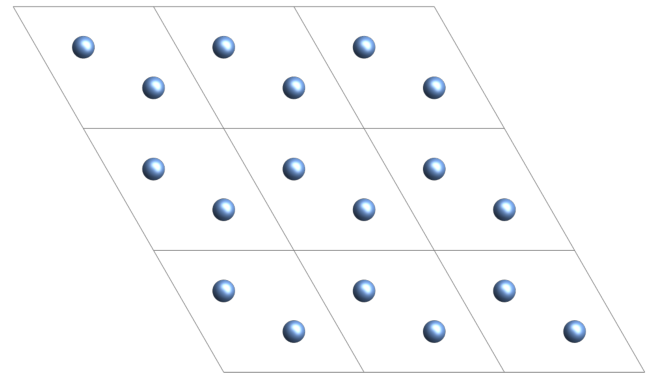
\includegraphics[width=.48\textwidth]{figures/manual-graphene-structure.pdf}
\hfill
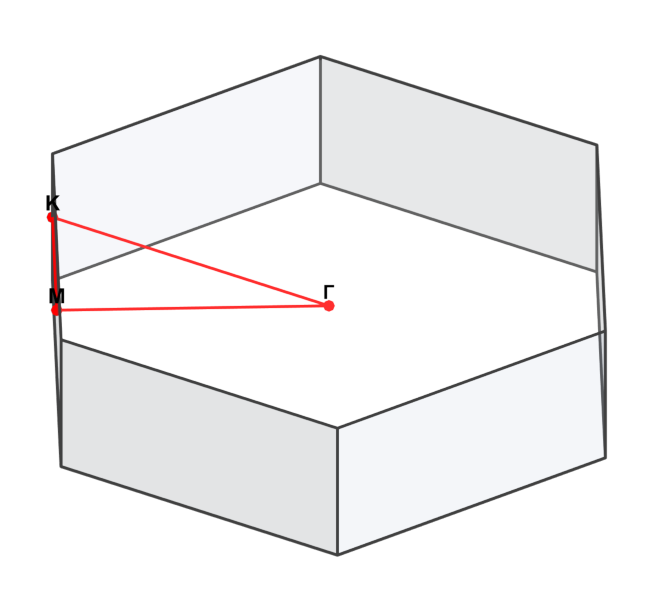
\includegraphics[width=.48\textwidth]{figures/manual-graphene-bz.pdf}
\caption{Atomic arrangement of graphene (left) and its first Brillouin zone
(right). The top view contains 18 carbon atoms. The path in the right panel
lies in the $k_z=0$ plane.}
\label{fig:graphene-structure}
\end{figure}

After checking the structure, generate the Hamiltonian with onsite,
nearest-neighbor, and second-neighbor terms:
\begin{lstlisting}
ham = Sum[symham[i], {i, 3}];
MatrixForm[ham]
\end{lstlisting}
The two rows correspond to the $p_z$ orbitals of the two carbon atoms.
The diagonal entries contain the onsite energy and second-neighbor hoppings
within each sublattice. The off-diagonal entries come from nearest-neighbor
hoppings between the two sublattices. Here \lstinline|e1| is the common onsite
energy, while \lstinline|t1| and \lstinline|r1| control the nearest- and
second-neighbor hoppings, respectively.

Combining the exponential terms gives
\[
H(\boldsymbol k)=\begin{pmatrix}d(\boldsymbol k)&t_1 f(\boldsymbol k)\\
t_1 f(\boldsymbol k)^*&d(\boldsymbol k)\end{pmatrix},
\]
where
\begin{align*}
d(\boldsymbol k)&=e_1+2r_1[\cos k_x+\cos k_y+\cos(k_x+k_y)],\\
f(\boldsymbol k)&=e^{i(k_x-k_y)/3}(1+e^{-ik_x}+e^{ik_y}).
\end{align*}
The three exponential terms come from the three nearest-neighbor bonds.
They cancel at $K$, where the two bands cross.

Once the parameters have been assigned, a single plotting command gives the
band structure:
\begin{lstlisting}
parameters = {e1 -> 0.05, t1 -> 0.5, r1 -> 0.02};
bandplot[path, 80, ham, parameters, ImageSize -> 440, FontSize -> 16]
\end{lstlisting}
\begin{figure}[H]
\centering
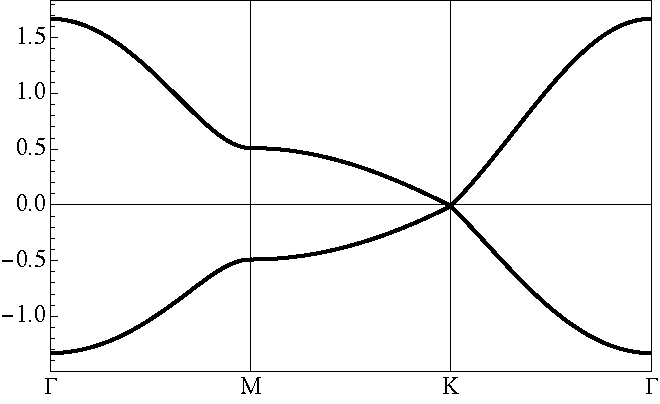
\includegraphics[width=.72\textwidth]{figures/manual-graphene-band.pdf}
\caption{The two $p_z$ bands of graphene for $e_1=0.05$, $t_1=0.5$, and
$r_1=0.02$. The bands cross at $K$. Second-neighbor hopping changes the
dispersion but does not open a gap at this crossing.}
\label{fig:graphene-band}
\end{figure}
The energy unit follows the parameter units: parameters entered in eV give
energies in eV. To explore how the parameters affect the bands, run:
\begin{lstlisting}[numbers=none]
bandManipulate[path, 80, ham]
\end{lstlisting}
Adjust the \lstinline|t1| and \lstinline|r1| sliders in the notebook to see the
changes.

The model can also be exported directly:
\begin{lstlisting}[numbers=none]
hop[3, parameters, "hrExport" -> "/absolute/path/graphene_hr.dat"]
\end{lstlisting}
There is no need to print the entire hopping table. If you want to inspect
the atoms and distances for a particular neighbor group, use
\lstinline|showbonds[2]| or \lstinline|showbonds[3]| separately.

\subsubsection{Including spin-orbit coupling}
To include spin-orbit coupling (SOC), replace each carbon $p_z$ orbital with
the two basis functions $p_z\uparrow$ and $p_z\downarrow$.
The complete initialization is:
\begin{lstlisting}
init[
  lattice -> {
    {a, 0, 0}, {-a/2, Sqrt[3] a/2, 0}, {0, 0, c}
  },
  lattpar -> {a -> 1, c -> 3},
  wyckoffposition -> {{{1/3, 2/3, 0}, {0, 0, 0}}},
  symminformation -> sgop,
  basisFunctions -> {{"pzup", "pzdn"}}
];
hamsoc = Sum[symham[i], {i, 3}];
MatrixForm[hamsoc]
\end{lstlisting}
The matrix now has four rows: the two spin states of the first carbon atom,
followed by those of the second. The lattice, positions, and space group are
unchanged, but the package constructs double-group representations in the
spinor basis. Simply copying the earlier two-band Hamiltonian twice does not
produce the SOC model.

In this four-band model, \lstinline|r1| controls spin-dependent second-neighbor
hopping and \lstinline|r2| controls spin-independent second-neighbor hopping.
Note that \lstinline|r1| no longer has the meaning it had in the two-band model.
Compare the bands with the SOC parameter set to 0 and 0.05:
\begin{lstlisting}
bandplot[
  path, 80, hamsoc, {e1 -> 0.05, t1 -> 0.5, r1 -> 0, r2 -> 0.02},
  ImageSize -> 440, FontSize -> 16
]
bandplot[
  path, 80, hamsoc, {e1 -> 0.05, t1 -> 0.5, r1 -> 0.05, r2 -> 0.02},
  ImageSize -> 440, FontSize -> 16
]
\end{lstlisting}
\begin{figure}[H]
\centering
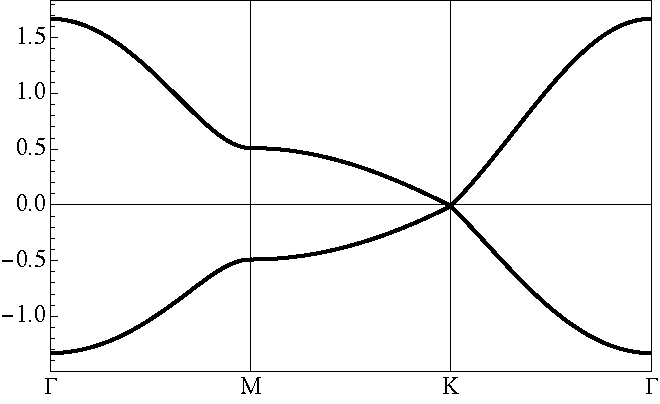
\includegraphics[width=.48\textwidth]{figures/manual-graphene-soc-off.pdf}
\hfill
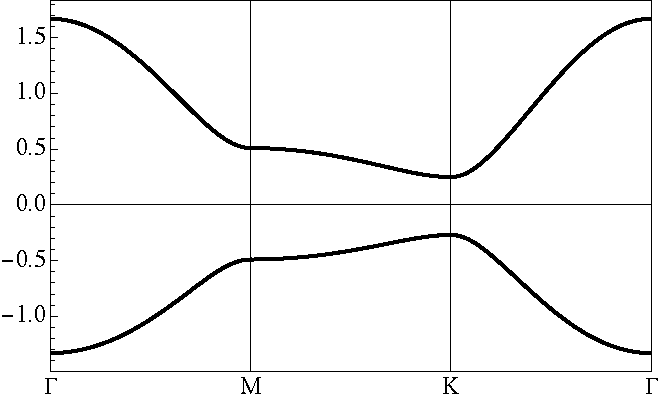
\includegraphics[width=.48\textwidth]{figures/manual-graphene-soc-on.pdf}
\caption{The same four-band graphene model with the SOC parameter set to 0
(left) and 0.05 (right). SOC opens a gap at $K$ in the right panel.
Each visible band remains doubly degenerate.}
\label{fig:graphene-soc}
\end{figure}

\subsection{Induced representations in a cubic lattice}
\label{sec:induced}
In some models, we want to retain only one $p$ orbital along a local axis at
each atom. Cubic rotations, however, can transform $p_x$ into $p_y$ or $p_z$.
If the same fixed local basis is used at every atom, all three orbitals
$p_x,p_y,p_z$ must be supplied.
The induced mode instead starts from a single $p_x$ at a reference atom and
uses symmetry to determine the orbitals at the equivalent atoms.

For example, the position $(1/2,0,0)$ in space group 221 generates three
equivalent sites. To retain only $p_x$ at the reference site, use:
\begin{lstlisting}
Needs["MagneticTB`"];
init[
  lattice -> {{a, 0, 0}, {0, a, 0}, {0, 0, a}},
  lattpar -> {a -> 1},
  wyckoffposition -> {{{1/2, 0, 0}, {0, 0, 0}}},
  symminformation -> msgop[gray[221]],
  basisFunctions -> {{"px"}},
  RepresentationMode -> "Induced"
];
orbitalTable[]
\end{lstlisting}
The option \lstinline|RepresentationMode -> "Induced"| selects the induced
mode. The three rows of the orbital table are, in order, $p_x$ at $(1/2,0,0)$,
$p_z$ at $(0,0,1/2)$, and $p_y$ at $(0,1/2,0)$.
The same $p_x$ orbital has not been placed on all three atoms.
Cubic rotations determine the orbital directions at the other two sites.

Plot the structure and the bands of the nearest-neighbor model:
\begin{lstlisting}
showCrystalStructure[
  "CellRange" -> {{0, 1}, {0, 1}, {0, 1}}, ImageSize -> 440
]
hamCubic = Simplify[ComplexExpand[symham[1] + symham[2]]];
hamCubic // MatrixForm
pathCubic = standardKPath[];
bandplot[
  pathCubic, 60, hamCubic, {e1 -> 0, t1 -> -1},
  ImageSize -> 440, FontSize -> 16
]
\end{lstlisting}
\begin{figure}[H]
\centering
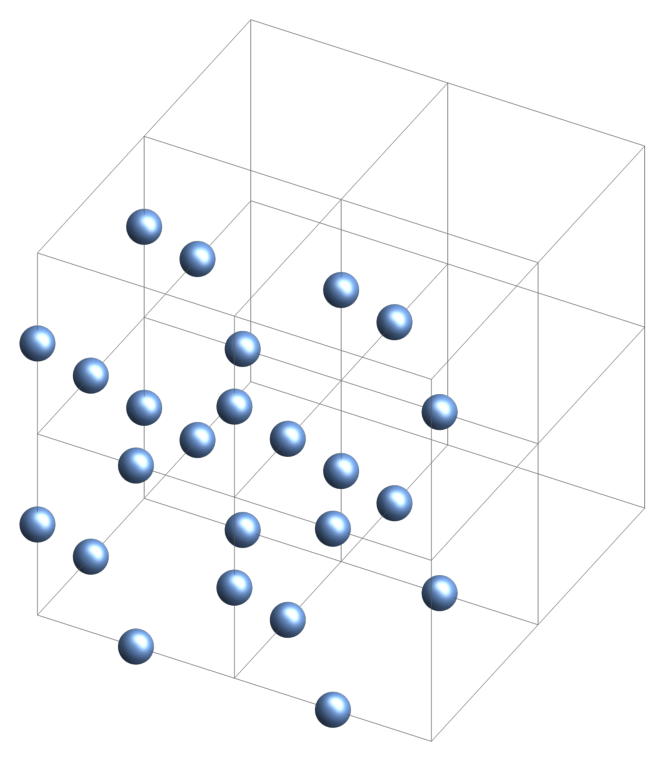
\includegraphics[width=.46\textwidth]{figures/manual-cubic-structure.pdf}
\hfill
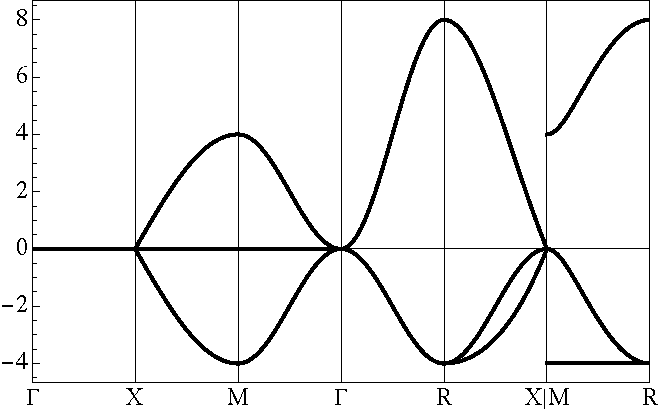
\includegraphics[width=.50\textwidth]{figures/manual-cubic-band.pdf}
\caption{Equivalent atoms in the cubic induced model (left) and its three
bands (right). Each atom carries one orbital obtained by transporting the
reference $p_x$. The structure plot shows atomic positions, not orbital lobes.}
\label{fig:cubic-induced}
\end{figure}
In the orbital order listed above, the matrix is
\[
H(\boldsymbol k)=e_1 I_3-4t_1
\begin{pmatrix}
0&s_xs_z&s_xs_y\\s_xs_z&0&s_ys_z\\s_xs_y&s_ys_z&0
\end{pmatrix},\qquad s_i=\sin(k_i/2).
\]
All three bands therefore coincide at $e_1$ along $\Gamma$--$X$.
Along $X$--$M$, two bands disperse upwards and downwards, while the third
remains at $e_1$. The label $X|M$ marks a jump from $X$ to $M$ before the next
segment; those two points are not connected.

To use the default \lstinline|"DirectProduct"| mode instead, replace the
last two options in the same complete initialization with:
\begin{lstlisting}[numbers=none]
basisFunctions -> {{"px", "py", "pz"}},
RepresentationMode -> "DirectProduct"
\end{lstlisting}
Now each of the three atoms has three orbitals, giving a nine-band model.
This is not the same basis as the three-band model above, so the complete
band structures should not be expected to match.
Induction lets you supply only the local states needed at the reference site;
it does not arbitrarily remove six bands from a nine-band model.

If another program already supplies the local representation matrices, use
\lstinline|initfromrep|. This function accepts representation matrices rather
than orbital strings. It requires a complete group in a fixed order and does
not accept \lstinline|GenerateSymmetryGroup|.
It is not needed for ordinary orbital-based modeling.

\subsection{A noncollinear magnetic kagome model}
\label{sec:kagome}
Consider a kagome model with three in-plane magnetic moments separated by
$120^\circ$. Their sum is zero, but each atom has a nonzero moment, so this
is not a nonmagnetic model. Use magnetic space group $191.239$ and supply a
local spinor at the reference site:
\begin{lstlisting}
Needs["MagneticTB`"];
init[
  lattice -> {
    {a, 0, 0}, {-a/2, Sqrt[3] a/2, 0}, {0, 0, c}
  },
  lattpar -> {a -> 1, c -> 4},
  wyckoffposition -> {{{1/2, 0, 0}, {1, 0, 0}}},
  symminformation -> msgop[typeIII[{191, 239}]],
  basisFunctions -> {{{1, -1}/Sqrt[2]}},
  RepresentationMode -> "Induced"
];
\end{lstlisting}
Here \lstinline|typeIII[{191,239}]| specifies this type-III magnetic space
group by its BNS number.
The two components of \lstinline|{1,-1}/Sqrt[2]| are expressed in the spin
$\uparrow,\downarrow$ basis. Together they describe \textbf{one} local state,
not two independent basis functions.
Induction transports this state to the other two equivalent sites, giving
three bands rather than the full six-band spinful model.

The generated positions are $(1/2,0,0)$, $(0,1/2,0)$, and $(1/2,1/2,0)$,
in that order. Their moments, expressed in the lattice basis, are $(1,0,0)$,
$(0,1,0)$, and $(-1,-1,0)$. Since the in-plane lattice vectors form an angle
of $120^\circ$, these moments have equal Cartesian lengths and are separated
by $120^\circ$.

\subsubsection{Viewing the magnetic structure}
First plot $2\times2$ primitive cells, then a top view of $3\times3$ cells:
\begin{lstlisting}
showCrystalStructure[
  "CellRange" -> {{0, 1}, {0, 1}, {0, 0}},
  "MomentScale" -> 0.3, ImageSize -> 400
]
Show[
  showCrystalStructure[
    "CellRange" -> {{0, 2}, {0, 2}, {0, 0}},
    "MomentScale" -> 0.3, ImageSize -> 400
  ],
  ViewPoint -> {0, 0, 3}, ViewVertical -> {0, 1, 0}
]
\end{lstlisting}
\begin{figure}[H]
\centering
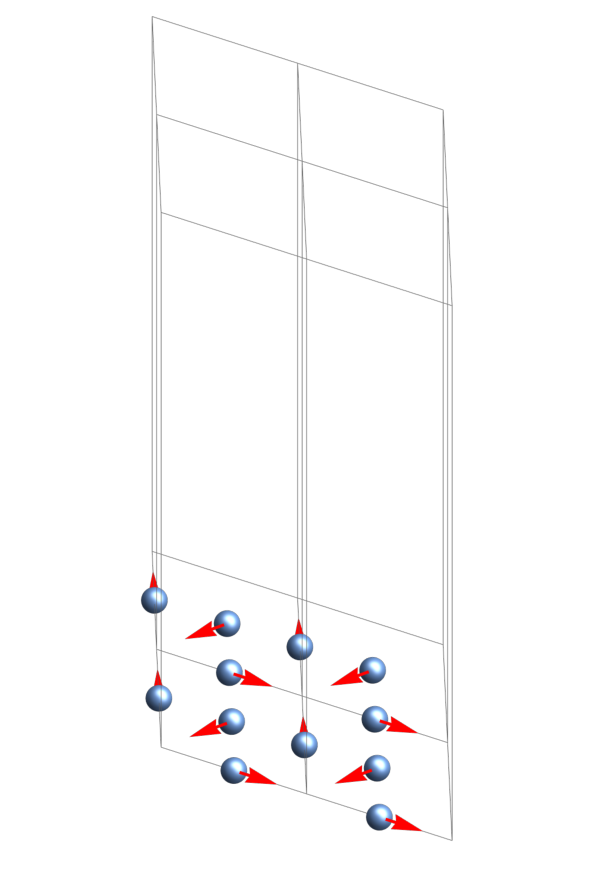
\includegraphics[height=.24\textheight]{figures/manual-kagome-structure.pdf}
\hfill
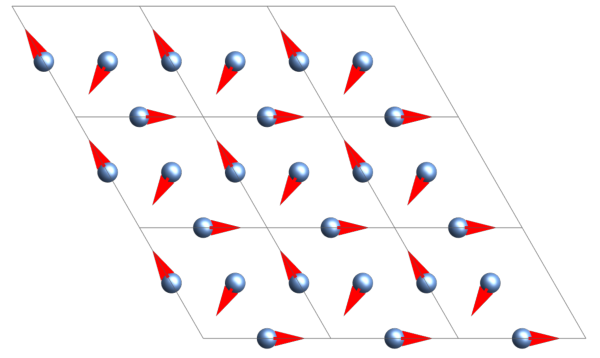
\includegraphics[width=.65\textwidth]{figures/manual-kagome-top.pdf}
\caption{Oblique view (left) and top view (right) of the noncollinear kagome
magnetic structure. The red arrows come directly from the initialized
magnetic moments. The three moment directions repeat throughout the top view.}
\label{fig:kagome}
\end{figure}
The option \lstinline|"MomentScale"| changes only the displayed arrow length,
not the magnetic moments in the model. Again, gray lines are cell boundaries,
not hopping paths.

\subsubsection{The Hamiltonian and bands}
This example includes only onsite and nearest-neighbor terms:
\begin{lstlisting}
kagomeHamiltonian = Simplify[ComplexExpand[symham[1] + symham[2]]];
kagomeHamiltonian // MatrixForm
\end{lstlisting}
For real momenta, \lstinline|ComplexExpand| and \lstinline|Simplify| rewrite
pairs of exponentials as cosines without changing the model.
The matrix is
\[
H(\boldsymbol k)=
\begin{pmatrix}
 e_1 & 2t_1\cos\frac{k_x+k_y}{2} & 2t_1\cos\frac{k_y}{2}\\
 2t_1\cos\frac{k_x+k_y}{2} & e_1 & -2t_1\cos\frac{k_x}{2}\\
 2t_1\cos\frac{k_y}{2} & -2t_1\cos\frac{k_x}{2} & e_1
\end{pmatrix}.
\]
The equal diagonal entries give the common onsite energy of the three
equivalent sites. The relative minus sign in the off-diagonal entries follows
from the chosen induced spinor basis; it must not be removed merely to make
the matrix look more uniform.

Use the $\Gamma$--$M$--$K$--$\Gamma$ path in the $k_z=0$ plane to plot the
Brillouin zone and bands:
\begin{lstlisting}
planePath = Take[standardKPath[], 3];
showBrillouinZone["KPath" -> planePath, ImageSize -> 400]
bandplot[
  planePath, 60, kagomeHamiltonian, {e1 -> 0, t1 -> -1},
  ImageSize -> 400, FontSize -> 16
]
\end{lstlisting}
\begin{figure}[H]
\centering
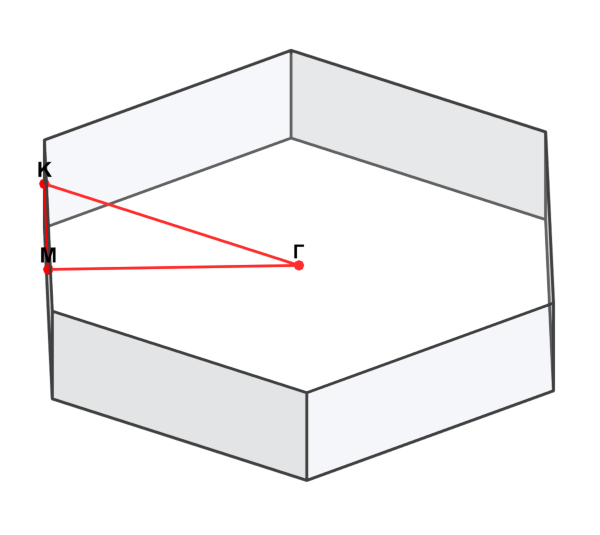
\includegraphics[width=.46\textwidth]{figures/manual-kagome-bz.pdf}
\hfill
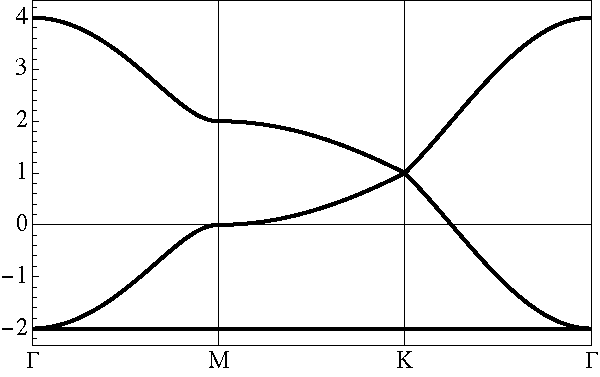
\includegraphics[width=.50\textwidth]{figures/manual-kagome-band.pdf}
\caption{In-plane path (left) and bands (right) of the same kagome model.
The flat band lies at $E=-2$, and the two dispersive bands meet at $K$ at $E=1$.}
\label{fig:kagome-band}
\end{figure}
At $\Gamma$, the flat band touches the lower dispersive band.
These two contributions contain no interlayer hopping, so the Hamiltonian
does not depend on $k_z$. This is an ideal magnetic kagome model.
Its parameters illustrate the symmetry-allowed bands; they are not a fit
to a particular material.

\section{Frequently asked questions}
\begin{enumerate}[style=nextline]
\setlength\itemsep{1.2em}

\litem{What if the help pages are not available after installation}
Answer: Use \lstinline|PacletFind["MagneticTB"]| to confirm the installation,
save your work, then quit and reopen Mathematica completely. Run
\lstinline|SystemOpen["paclet:MagneticTB/guide/MagneticTB"]|
to open the help home page. Restarting only the kernel can leave old help
pages open in the front end.

\litem{Why can init not construct a model from lattice constants alone}
Answer: Lattice constants set the geometric scale, but do not specify the
atomic positions, symmetry, or orbitals.
Provide all five model inputs as in Section~\ref{sec:init}.
A call such as \lstinline|init[lattice -> ...]| is not a complete model.

\litem{Do operations obtained from msgop need group completion}
Answer: No. The function \lstinline|msgop| already provides the complete
operation list, and \lstinline|GenerateSymmetryGroup| defaults to
\lstinline|False|. Add \lstinline|GenerateSymmetryGroup -> True|
to the complete initialization only when supplying generators yourself.

\litem{Why are all bands horizontal when bandManipulate first opens}
Answer: The sliders start at zero. With zero onsite energies and hoppings,
the Hamiltonian is the zero matrix. Set a hopping parameter to a nonzero
value, or use \lstinline|bandplot| with explicit parameter values, to see
the dispersion.

\litem{Why does the Hamiltonian expression change with the lattice basis}
Answer: Momentum coordinates, fractional atomic positions, and symmetry
operations all depend on the basis. For example, using in-plane angles of
$120^\circ$ and $60^\circ$ for a hexagonal lattice produces different
expressions for the same physical model. Before comparing results, put the
lattice, positions, operations, and momentum path into the same convention.
Comparing only parameter names or individual matrix elements is not sufficient.

\litem{When can the induced mode start from a single px orbital}
Answer: The local basis at the reference site must be closed under its
site-symmetry group. The cubic example in Section~\ref{sec:induced} satisfies
this condition and can start from one $p_x$ orbital.
A single component is not sufficient at every site for every orbital.
If a site-symmetry operation maps $p_x$ to another independent state, include
that state in the reference basis as well.

\litem{Can I remove a few parameters to keep spin but neglect SOC}
Answer: Parameter names alone do not determine which terms to remove.
\textsf{MagneticTB} supports separate spatial and spin actions, and the
explicit-representation interface can include one internal continuous spin
rotation $C_\infty$. A model without SOC should use spin-symmetry constraints
appropriate to the magnetic structure. See the \emph{Continuous spin symmetry}
tutorial for the construction, rather than setting arbitrary entries of an
SOC Hamiltonian to zero.

\litem{How can I calculate other physical properties}
Answer: Use the relevant property functions in the package, or export a
Wannier90 file with \lstinline|hop| for use in other software.
Functions can differ in their coordinate and orbital-center conventions.
Read the relevant help page first, and do not mix a hand-written momentum
function with the default $H(\boldsymbol k)$ convention.

\litem{How do I use version 1.0}
Answer: In a fresh kernel, run \lstinline|Needs["MagneticTBOld`"]|,
then use \lstinline|initold|, \lstinline|symhamold|, and the other version-1.0
functions. Load versions 1.0 and 2.0 in separate kernels.
See the \emph{Using MagneticTB 1.0} tutorial for complete inputs.

\newpage
\litem{Where can I find more examples}
Answer: After installing the paclet, open the \emph{MagneticTB general examples},
\emph{Crystal structure, Brillouin zone, and k paths}, or band-fitting tutorials
from the help home page. Function pages also show how to use their options.
You can adapt the example parameters to your own model.

\litem{How can I report a problem}
Answer: Join QQ group 625192239, open an issue at
\url{https://github.com/zhangzeyingvv/MagneticTB/issues},
or email \href{mailto:zhangzeyingvv@gmail.com}{zhangzeyingvv@gmail.com}.
Include the package version, complete input, and error messages so that the
problem can be reproduced.
\begin{figure}[H]
\centering
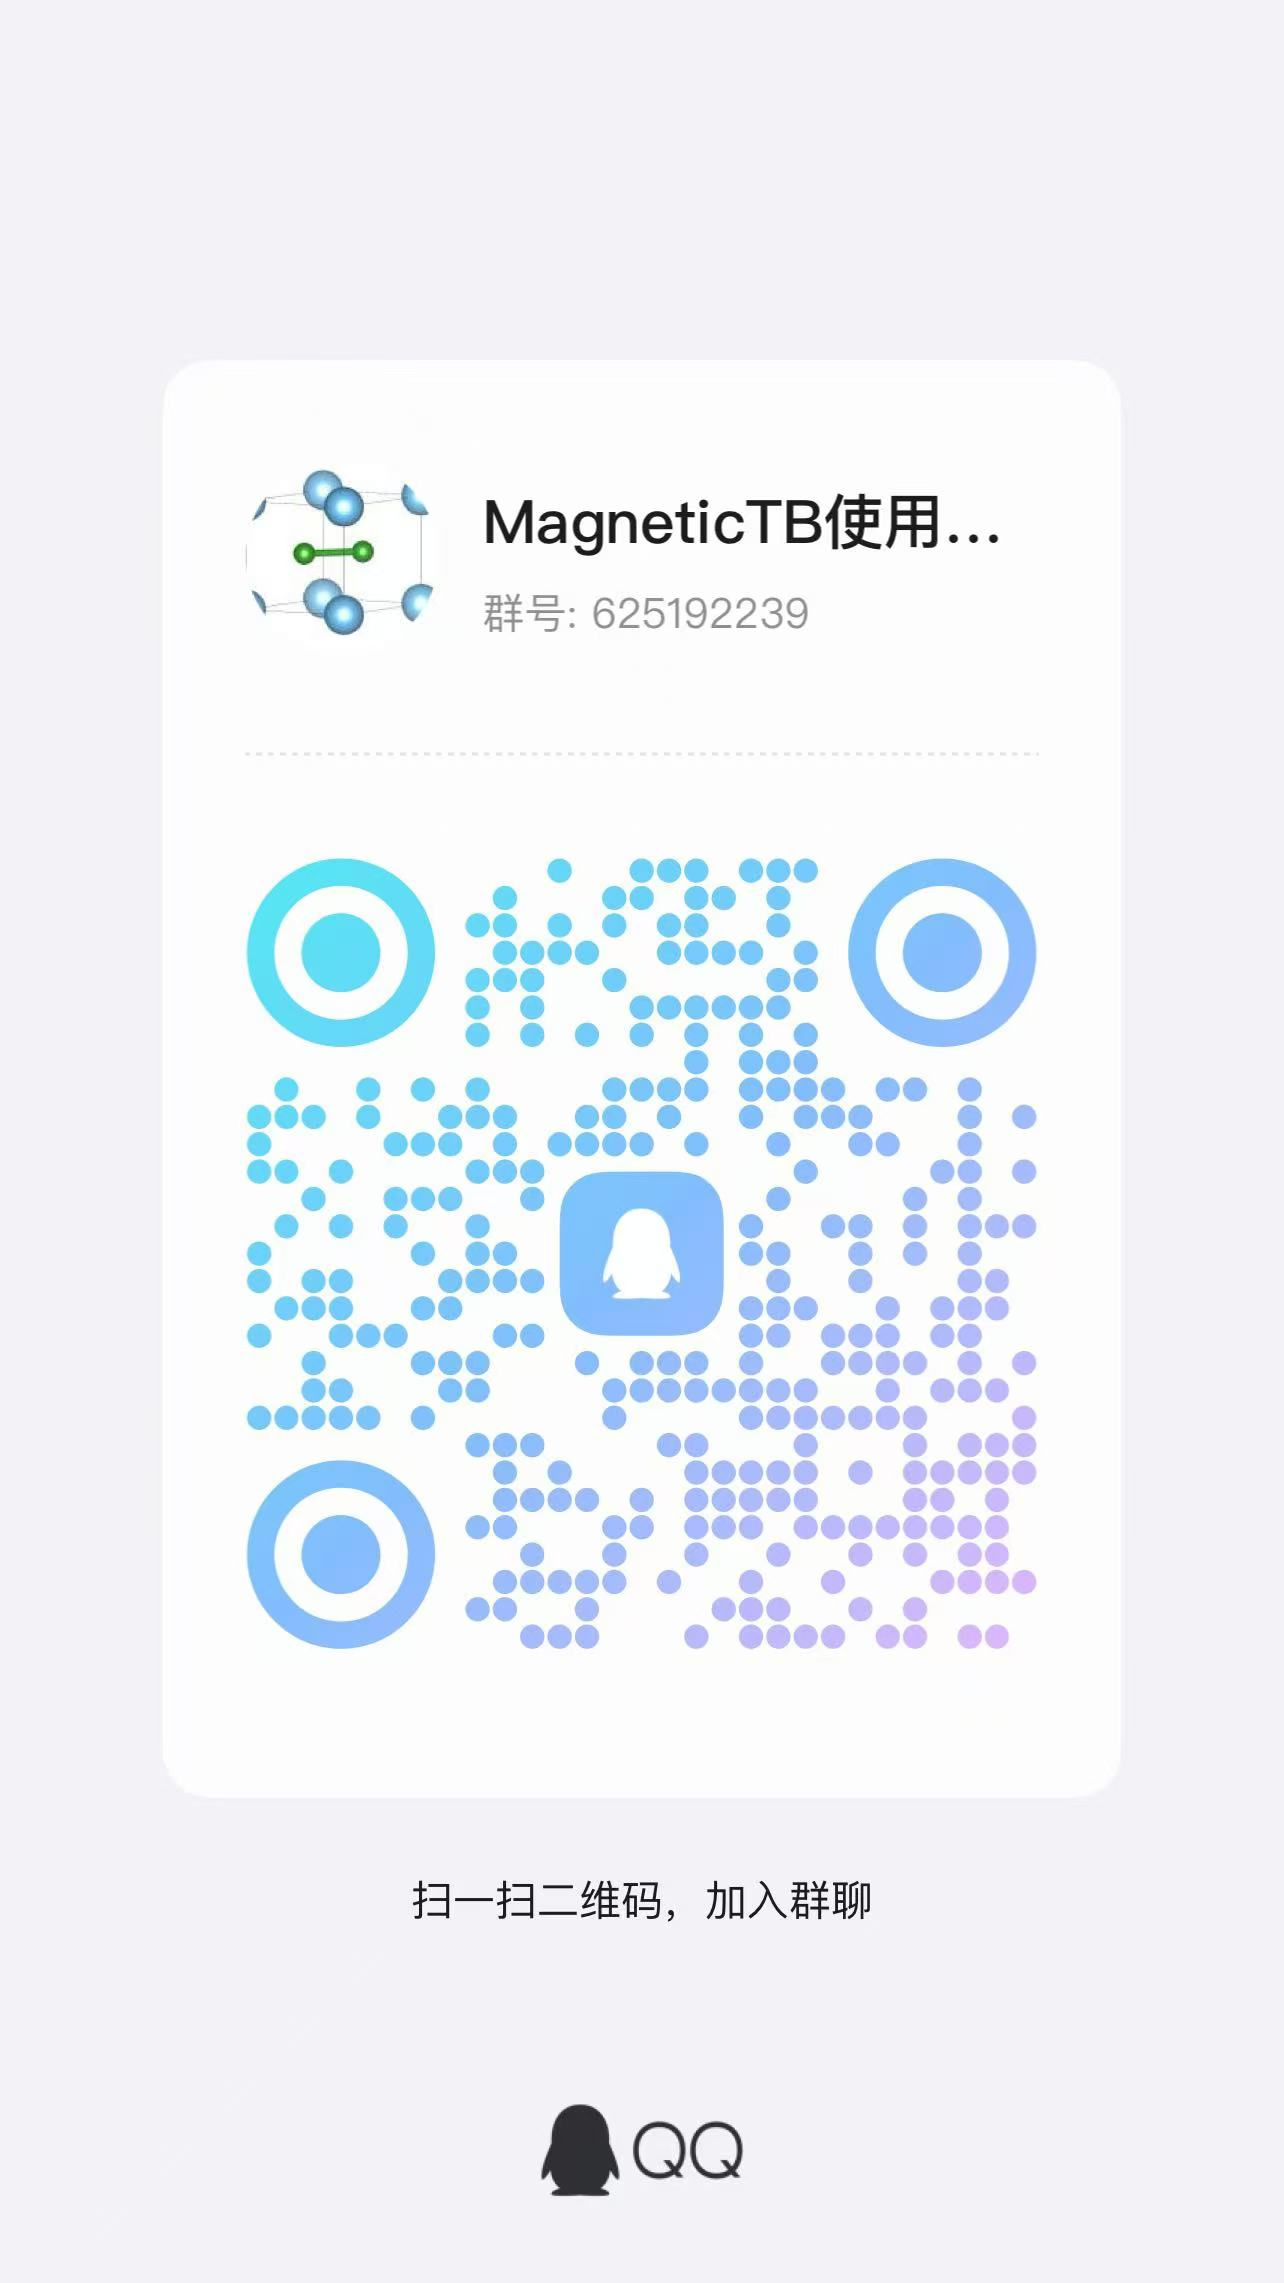
\includegraphics[width=.23\textwidth]{figures/QQ.jpg}
\end{figure}

\litem{How should I cite MagneticTB}
Answer: If you use the package in your research, please cite:
Zeying Zhang, Zhi-Ming Yu, Gui-Bin Liu, Yugui Yao,
\textit{MagneticTB: A package for tight-binding model of magnetic and non-magnetic materials},
Computer Physics Communications \textbf{270}, 108153 (2022).
DOI: \href{https://doi.org/10.1016/j.cpc.2021.108153}{10.1016/j.cpc.2021.108153}.
\begin{lstlisting}[numbers=none,language=TeX]
@article{ZHANG2022108153,
  title = {MagneticTB: A package for tight-binding model
    of magnetic and non-magnetic materials},
  author = {Zhang, Zeying and Yu, Zhi-Ming and
    Liu, Gui-Bin and Yao, Yugui},
  journal = {Computer Physics Communications},
  volume = {270},
  pages = {108153},
  year = {2022},
  doi = {10.1016/j.cpc.2021.108153}
}
\end{lstlisting}
\end{enumerate}
\end{document}
